\section{Introduction}
\label{section:intro}
Although enormous amounts of data exist in ``well-behaved'' formats such
as relational tables and XML, massive amounts also exist in
non-standard or \textit{ad hoc} data formats. \tblref{figure:data-sources}
gives some sense of the range and pervasiveness of such data.
Ad hoc data comes in many forms: ASCII, binary, EBCDIC, and mixed
formats.  It can be fixed-width, fixed-column, variable-width, or even
tree-structured.  It is often quite large, including some data sources
that generate over a gigabit per second~\cite{gigascope}. It frequently
comes with incomplete and/or out-of-date documentation, and there are
almost always errors in the data.  Sometimes these errors are the most
interesting aspect of the data, \eg{}, in log files where
errors indicate that something is going wrong in the associated
system.

\begin{table}
\begin{center}
\begin{tabular}{l|l}
\hline
\textbf{Name} : Use   &  Representation               \\ \hline
\textbf{Web server logs (CLF)}:  &  Fixed-column ASCII records \\ 
Measure web workloads &                             \\ \hline
\textbf{AT\&T provisioning data}: & Variable-width ASCII records  \\ 
Monitor service activation &                              \\ \hline
\textbf{Call detail}: Fraud detection  &  Fixed-width binary records \\  \hline 
\textbf{AT\&T billing data}: & Various Cobol data formats  \\ 
Monitor billing process   &                             \\ \hline
\textbf{Netflow}:            & Data-dependent number of     \\ 
Monitor network performance  & fixed-width binary records  \\ \hline
\textbf{Newick}:   Immune  & Fixed-width ASCII records \\ 
system response simulation & in tree-shaped hierarchy\\ \hline                                
\textbf{Gene Ontology}:    & Variable-width ASCII records \\
Gene-gene correlations     & in DAG-shaped hierarchy \\ \hline
\textbf{OPRA}:              & Mixed binary \& ASCII records \\
Options-market transactions & with data-dependent unions \\ \hline
%IP backbone data:  & ASCII   \\
%Monitor network performance  &        \\ \hline
%HL7:             & Variable-width ASCII records \\
%Medical lab results     &  \\ \hline
% \textbf{CPT codes}: Medical diagnoses & Floating point numbers \\ \hline
% \textbf{SnowMed}: Medical clinic notes & Keyword tags  \\ 
\end{tabular}
\caption{Selected ad hoc data sources.}
\label{figure:data-sources}
\end{center}
\end{table}

The lack of standard tools for processing ad hoc data forces
analysts to roll their own tools, leading to scenarios such as the
following.  An analyst receives a new ad hoc data source containing
potentially interesting information and a list of pressing questions
about that data.  Could she please provide the answers to the
questions as quickly as possible, preferably last week?  The
accompanying documentation is outdated and missing important
information, so she first has to experiment with the data to discover
its structure.   Eventually, she understands the data well enough to hand-code a
parser, usually in \C{} or \perl{}.  Pressed for time, she interleaves
code to compute the answers to the supplied questions with the parser.
As soon as the answers are computed, she gets a new data source and a
new set of questions to answer.

Through her heroic efforts, the data analyst answered the necessary
questions, but the approach is deficient in many respects.  The
analyst's hard-won understanding of the data ended up embedded in a
hand-written parser, where it is difficult for others to benefit from
her understanding.  The parser is likely to be brittle with respect to
changes in the input sources.  Consider, for example, how tricky it is
to figure out which \$3's should be \$4's in a \perl{} parser when a
new column appears in the data.  Errors in the data also pose a
significant challenge in hand-coded parsers.  If the data analyst
thoroughly checks for errors, then the error checking code dominates
the parser, making it even more difficult to understand the semantics
of the data format.  If she is not thorough, then erroneous data can
escape undetected, potentially (silently!)  corrupting down-stream
data processing.  Finally, during the initial data exploration and in
answering the specified questions, the analyst had to code \textit{how
to compute} the questions rather than being able to express the
queries in a declarative fashion.  Of course, many of these pitfalls
can be avoided with careful design and sufficient time, but such
luxuries are not available to the analyst.  However, with the
appropriate tool support, many aspects of this process can be greatly
simplified.

The \pads{} system~\cite{fisher+:pldi05} allows analysts to describe
ad hoc data sources declaratively.  The descriptions take the form of
types, drawn from a dependent type theory~\cite{fisher+:popl06}.
\pads{} base types describe simple objects including strings,
integers, floating-point numbers, dates, times, and IP addresses.
Records and arrays specify sequences of elements in a data source, and
unions, switched unions, and enums specify alternatives.  Any of these
structured types may be parameterized, and users may write arbitrary
semantic constraints as well.  The \pads{} language is both expressive
and concise.  \pads{} descriptions exist for all the data sources in
\tblref{figure:data-sources}, and 92 pages of the OPRA standard is
captured by a 450-line \pads{} description.

The \pads{} compiler produces a customizable, error-aware library for
parsing a given ad hoc data source.  A suite of tools built around
this library include statistical data-profiling tools, such as
histograms, accummulators and clustering algorithms; a query engine
that permits viewing ad hoc sources as XML and for querying them with
XQuery~\cite{fernandez+:padx}; and an interactive front-end that helps
users produce \pads{} descriptions and invoke tools without having to
learn nitty-gritty details of the \pads{} language or tool interfaces.

\section{Using PADS}
\label{subsec:example}

In our demonstration, we will present a scenario similar to the
following, in which an AT\&T data analyst interactively creates a
\pads{} description for a new data source, uses \pads{} tools to learn
about the distribution of values and errors in her data, and writes
and executes simple queries to perform basic analysis tasks.  A
shorter version of this demonstration proposal was accepted to the PLAN-X
2006 workshop~\cite{daly+:launchpads}.

Our analyst's task is to process \textit{provisioning} data.  In the
telecommunications industry, the term {provisioning} refers to
the complex, inter-company process of converting an order for phone
service into the actual service.  In practice, AT\&T's \dibbler{}
project discovers provisioning problems proactively by compiling
weekly summaries of the state of phone service
orders.  These summaries, which are stored in flat ASCII text files,
can contain more than 2.2GB of data per
week. \figref{figure:dibbler-records} contains sample \dibbler{} data
provided to our analyst.
\begin{figure*}
\begin{small}
\begin{center}
\begin{verbatim}
0|15/Oct/2004:18:46:51
9152|9152|1|9735551212|0||9085551212|07988|no_ii152272|EDTF_6|0|APRL1|DUO|10|16/Oct/2004:10:02:10
9153|9153|1|0|0|0|0||152268|LOC_6|0|FRDW1|DUO|LOC_CRTE|1001476800|LOC_OS_10|17/Oct/2004:08:14:21
\end{verbatim}
\caption{Tiny example of \dibbler{} provisioning data.}
\label{figure:dibbler-records}
\end{center}
\end{small}
\end{figure*}

Provisioning summaries store the processing date and one record
per order.  Each order record contains a header followed by a nested
sequence of events.  The header has 13 pipe separated fields: the
order number, AT\&T's internal order number, the order version, four
different telephone numbers associated with the order, the zip code, a
billing identifier, the order type, a measure of the complexity of the
order, an unused field, and the source of the order data.  Many of
these fields are optional, in which case nothing appears between the
pipe characters.  The billing identifier may not be available at the
time of processing, in which case the system generates a unique
identifier, and prefixes this value with the string ``no\_ii'' to
indicate the number was generated. The event sequence represents the
various states a service order goes through; it is represented as a
new-line terminated, pipe separated list of state, timestamp pairs.
There are over 400 distinct states that an order may go through during
provisioning.  It may be apparent from this description that English
is a poor language for describing data formats!  If lucky, our analyst
might be provided with a formal specification of this format, but
often such specifications are incomplete or outdated.  If unlucky, she
might have only an informal description such as the above.

The analyst's first task is to write a parser for the \dibbler{} data
format.  Like many ad hoc data sources, \dibbler{} data can contain
unexpected or corrupted values, so the parser must handle errors
robustly to avoid corrupting the results of analyses.  With \pads{},
the analyst writes a declarative data description of the physical
layout of her data.  The language also permits the analyst to describe
expected semantic properties of her data so that deviations can be
flagged as errors. The intent is to allow an analyst to capture in a
\pads{} description all that she knows about a given data source.

If the analyst is new to \pads{}, she can use the interactive user
interface shown in \figref{figure:launchpads} to help create a \pads{}
description.  She begins by loading her sample \dibbler{} data into
the {\it dataview} (top-right frame) and then selects a fragment of
data to describe in the {\it gridview} (middle frame).  In the
gridview, the analyst iteratively refines the description of the
selected data.  In this example, she has selected the \scream{XXX}
part of an order record and is defining its composite structure, which
includes \scream{YYY}.  This refinement step terminates when the
analyst has associated an atomic type, such as character string, phone
number, or date, with every value in the sample data.  Once all
selected values have an associated base type, \textsc{LaunchPADS}
generates the {\it treeview} (left-hand frame).  The treeview depicts
the abstract syntax of a \pads{} description.  In this view, the
analyst can refine the description by creating, removing,
reordering, or renaming the generated types.

When the analyst is satisfied with the definition in the
treeview, they may generate \pads{} code.  Any such generated code is
guaranteed to be syntactically correct so the user need not worry
about fussing with concrete \pads{} syntax.
Figure~\ref{figure:launchpads} shows the generated code in bottom-most
frame.

By using the pulldown menus at the top and a set of
``wizards,'' the user may now
issue commands to compile the generated code and create data processing
tools including the XML converter and statistical analyzer.  

\begin{figure*}
  \begin{center}
    \scalebox{.75}{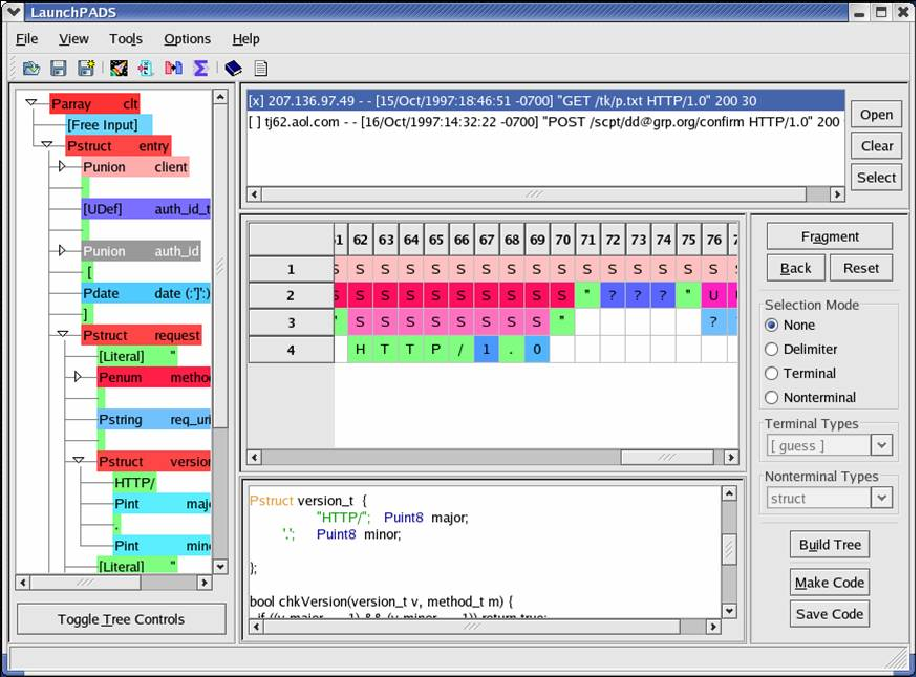
\includegraphics{launch.pdf}}
  \end{center}
  \caption{LaunchPADS Interactive User Interface.}
  \label{figure:launchpads}
\end{figure*}

\figref{figure:dibbler} gives the \pads{} description for the
\dibbler{} data format.  In \pads{} descriptions, types are declared
before they are used, so the type that describes the entire data
source, \cd{summary\_t}, appears at the bottom of the description (Line~42).  In
the next section, we use this example to give an overview of
the \pads{} language.  Here, we simply note that the data analyst
writes this description, and the \pads{} compiler produces
customizable \C{} libraries and tools for parsing, manipulating, and
summarizing the data.  The fact that useful software artifacts are
generated from \pads{} descriptions provides strong incentive for
keeping the descriptions current, allowing them to serve as living
documentation.

\begin{figure}
\begin{small}
\begin{code}
{ 1}. \kw{Precord} \kw{Pstruct} summary\_header\_t \{
{ 2}.  "0|";
{ 3}.  Punixtime tstamp;
{ 4}. \};
\mbox{}
{ 5}. \kw{Pstruct} no\_ramp\_t \{
{ 6}.  "no\_ii";
{ 7}.  Puint64 id;
{ 8}. \};
\mbox{}
{ 9}. \kw{Punion} dib\_ramp\_t \{
{10}.   Pint64     ramp;
{11}.   no\_ramp\_t  genRamp;
{12}. \};
\mbox{}
{13}. \kw{Pstruct} order\_header\_t \{
{14}.        Puint32             order\_num;
{15}.  '|';  Puint32             att\_order\_num;
{16}.  '|';  Puint32             ord\_version;
{17}.  '|';  \kw{Popt} pn\_t           service\_tn;
{18}.  '|';  \kw{Popt} pn\_t           billing\_tn;
{19}.  '|';  \kw{Popt} pn\_t           nlp\_service\_tn;
{20}.  '|';  \kw{Popt} pn\_t           nlp\_billing\_tn;
{21}.  '|';  \kw{Popt} Pzip           zip\_code;
{22}.  '|';  dib\_ramp\_t          ramp;
{23}.  '|';  Pstring(:'|':)      order\_type;
{24}.  '|';  Puint32             order\_details;
{25}.  '|';  Pstring(:'|':)      unused;
{26}.  '|';  Pstring(:'|':)      stream;
{27}. \};
\mbox{}
{28}. \kw{Pstruct} event\_t \{
{29}.        Pstring(:'|':)    state;   
{30}.   '|'; Punixtime         tstamp;
{31}. \};
\mbox{}
{32}. \kw{Parray} event\_seq\_t \{
{33}.   event\_t[] : \kw{Psep}('|') && \kw{Pterm}(\kw{Peor});
{34}. \};
\mbox{}
{35}. \kw{Precord} \kw{Pstruct} order\_t \{
{36}.        order\_header\_t  order\_header;
{37}.   '|'; event\_seq\_t     events;
{38}. \};
\mbox{}
{39}. \kw{Parray} orders\_t \{
{40}.   order\_t[];
{41}. \};
\mbox{}
{42}. \kw{Psource} \kw{Pstruct} summary\_t\{
{43}.   summary\_header\_t  summary\_header;
{44}.   orders\_t          orders;
{45}. \};
\end{code}
\end{small}
\caption{\pads{} description for \dibbler{} provisioning data.}
\label{figure:dibbler}
\end{figure}

Analysts working with ad hoc data often want to query their data.  
Questions posed by the \dibbler{} analyst include ``Select all
orders starting within a certain time window,'' ``Count the number of
orders going through a particular state,'' and ``What is the average
time required to go from a particular event state to another
particular event state''.  Such queries are useful for rapid
information discovery and for vetting errors and anomalies in data
before that data proceeds to a down-stream process or is loaded into a 
database.

\begin{figure}
\begin{small}
\begin{code}
\kw{(: Return orders started in October 2004 :)}
$pads/Psource/orders/elt[events/elt[1]
  [tstamp/rep {>=} {xs:dateTime}("2004-10-01:00:00:00")
{and} tstamp/rep {<} {xs:dateTime}("2004-11-01:00:00:00")]]
\end{code}
\end{small}
\caption{Query applied to \dibbler{} provisioning data.}
\label{figure:dibbler-query}
\end{figure}

With \pads{}, the analyst writes declarative XQuery expressions to
query her ad hoc data source.  Because XQuery is designed to
manipulate semi-structured data, its expressiveness matches ad hoc
data sources well.  As a Turing-complete language, XQuery is powerful
enough to express all the questions above.  For example,
Figure~\ref{figure:dibbler-query} contains an XQuery expression that
produces all orders that started in October, 2004.

\eat{One benefit is that XQuery queries may be
statically typed, which helps detect common errors at compile time.
For example, static typing would raise an error if the path expression
in Figure~\ref{figure:dibbler-query} referred to \cd{ordesr} instead
of \cd{orders}, or if the analyst erroneously compared the timestamp
value in \cd{tstamp} to a string.}

\eat{\begin{verbatim}
[Term]
id: GO:0000001
name: mitochondrion inheritance
namespace: biological\_process
def: "The distribution of mitochondria, including the mitochondrial
genome, into daughter cells after mitosis or meiosis, mediated by
interactions between mitochondria and the cytoskeleton."
[PMID:10873824, PMID:11389764, SGD:mcc]
is_a: GO:0048308 ! organelle inheritance
is_a: GO:0048311 ! mitochondrion distribution
\end{verbatim}
\caption{Tiny example of Gene Ontology (go) data.}
\label{figure:go-data}}
